\cleardoublepage
% ==============================================================
\chapter{Introduction}
% ==============================================================

The availability of genome sequences is a key prerequisite for modern 
biological research.
Even before the discovery of the DNA double-helix structure by 
\citeauthor{Watson1953} in \citeyear{Watson1953}, the gene had for several 
decades been regarded as the central unit representing a 
`hereditary characteristic' \citep{Vries1889} and therefore was considered
to play a major role in elucidating one of the biggest mysteries of nature, 
life itself.
After \citeauthor{Jou1972} published the first bacteriophagic nucleotide 
sequence for a single gene in \citeyear{Jou1972}, more elaborate genome 
sequencing techniques have been developed and refined in the following years
\citep{Gilbert1973, Sanger1975, Maxam1977}, culminating in the publication of 
the full human genome sequence in 2001 \citep{Venter2001}.
The possibility to obtain genome sequences has added considerable momentum
to biological research and full genome sequences for more than 180 species
are available (\cite{Yates2009}, see Table \ref{tab:genome-sizes}).
Interestingly, the number of genes encoded in a genome does not seem to strongly
correlate to the size of the genome.
For example, the number of human genes was initially overestimated to be around 
2 million \citep{Kauffman1969}.
More recent studies estimate the human genome to comprise about 20,000 -- 25,000 
genes, with protein diversity being achieved through alternative splicing 
\citep{Rubin2004}.
Aside from the ambiguities introduced by alternative splicing of genes 
\citep{Black2003} and non-coding regions in the genome \citep{Gilbert1978},
the genome provides -- in theory -- all necessary information about which 
proteins can potentially be expressed in a cell.
However, the amino acid sequence of a protein alone does not determine the 
final function of the protein.
Post-translational modifications or conformational changes, facilitated by
chaperone proteins, may be necessary for protein activation.
Furthermore, metabolic pathways and protein-protein interaction cannot be
investigated on the genomic level alone.
Apparently, in order to study the dynamic nature of a cell or organism, as for 
example in response to changing environmental conditions, the static information
provided by the genome is not sufficient. 

\begin{table}
\begin{tabular}{|l|r|r|l|}
\hline
Species & Genome size & Predicted genes & Reference \\
\hline
{\em Escherischia coli} & 5 Mbp & $\sim$5,400 & \cite{Welch2002} \\
{\em Thalassiosira pseudonana} & 34 Mbp & $\sim$11,200 & \cite{Armbrust2004} \\
{\em Arabidopsis thaliana} & 119 Mbp & $\sim$25,500 & \cite{Arabidopsis2000} \\
{\em Chlamydomonas reinhardtii} & 121 Mbp & $\sim$15,100 & \cite{Merchant2007} \\
{\em Drosophila melanogaster} & 165 Mbp & $\sim$13,600 & \cite{Adams2000} \\
{\em Daphnia pulex} & 200 Mbp & $\sim$30,900 & \cite{Colbourne2011} \\
{\em Homo sapiens} & 3.2 Gbp & $\sim$20,300 & \cite{Venter2001} \\
\hline
\end{tabular}
\caption{{\bf Genome sizes of selected species.} The range of known genome sizes 
    comprises several orders of magnitude, while the number of genes seems
    relatively unaffected by the genome size.
}
\label{tab:genome-sizes}
\end{table}

\paragraph{Omics-based approaches.}

Since the beginning of the current century the copious amounts of large-scale 
genome sequencing data have spurred a number of {\em omics}-related areas of 
research \citep{Sauer2007, Colquhoun2005}.
Originating from genomics, which deals with the effects of genes on the 
development and control of biological processes, several related {\em omics} 
fields of research have emerged.
The field of {\em functional
genomics} deals with the elucidation of dynamic aspects of genes in regard
to whole genomes \citep{Hieter1997}.
Likewise, the field of {\em structural genomics} attempts to predict 
three-dimensional structures of all proteins encoded by a genome, also on
a genome-wide level \citep{Baker2001a}.
The role of environmental influences on the genome is addressed in the field
of {\em epigenomics} \citep{Jirtle2007}.
Taking a step away from the genome, the {\em transcriptome} is defined as the 
entire set of gene transcripts of a genome, and the research area of 
{\em transcriptomics} monitors the transcriptional regulation of genes.
DNA microarray techniques can be employed to screen the regulation of many
genes in parallel on the transcript level \citep{Schena1995}, in high throughput.
Common to all {\em omics} methods is the scope of the research -- typically, the 
analysis encompasses entire genomes.
This is in stark contrast to previous times when gene regulation and 
transcription, as well as protein function and structure have been analyzed on 
a per-gene or per-protein basis.
Just as the genome is a precursor to the transcriptome, the transcriptome can
be regarded as a precursor to the {\em proteome}.
The field of {\em proteomics} deals with the total set of proteins expressed in 
a cell, tissue, or organism, at a defined time point and under certain 
conditions \citep{Yarmush2002, Yates2009}.
The notion of the {\em proteome} was coined by Marc Wilkins in 1994 
to reflect the entire set of proteins that are encoded in a genome and are 
actually expressed by a cell \citep{Wilkins2009}.
Interestingly, transcriptional regulation does not always correlate to
protein expression in a linear fashion and \citep{Rogers2008}.
In particular, expression of a specific protein cannot be inferred from the 
presence of its transcript because it has been shown that sometimes, mRNA 
is not translated into a protein at all \citep{Eddy2001}.
Complementing genomics, transcriptomics, and proteomics, the field of
{\em metabolomics} deals with small molecules which are synthesized or
metabolized in a cell \citep{Kell2004}.

% The transcriptome can be regarded as a precursor of the proteome.
% However, transcriptional regulation does not necessarily correlate to
% protein expression in a linear fashion \citep{Rogers2008}.
% It is therefore vital to combine various types of qualitative and quantitative
% information, including the transcriptome and proteome, with further aspects such 
% as evolution and the modeling of interactions on the levels of molecules, 
% proteins, and cells to achieve a comprehensive understanding of life.
% In the past few years, this approach has manifested itself as {\em systems 
% biology} \citep{Vidal2009}.
% In addition to genomics, transcriptomics, and proteomics, further fields 
% involved in the holistic approach of systems biology include metabolomics,
% in which the end products of metabolic processes are analyzed 
% \citep{Daviss2005}.
% Furthermore, glycomics and lipidomics which provide a view on life from the
% perspective of carbohydrates and lipids, respectively, contribute to the
% overall picture in the systems biology framework.

\paragraph{Systems biology.}

The previously mentioned {\em omics}-related fields of research each deal
with a specific aspect of biology.
While the methods employed in these areas provide detailed insights on the 
molecular level, this information is not sufficient to gain a general 
understanding of biology on the the systems level \citep{Kitano2002}.
While comprehensive lists of genes and proteins, along with a mapping
of their relations represents a valuable foundation of knowledge which can
be built upon, a meta layer is required which is able to integrate the
different sources of molecular information.
An example provided by \citeauthor{Kitano2002} in his review uses an analogy 
to an airplane.
While a listing of all airplane parts is not sufficient to understand or even
build a functional airplane because information beyond the scope of individual
components is missing, for example regarding the assembly of the single parts,
how signals are encoded on signal lines, and how they can be made robust against
external influences, noise, and malfunction.

The field of {\em systems biology} attempts to provide a systems-level 
understanding of biology. 
To achieve this goal, large-scale data reporting on various aspects of a 
biological system is combined on several levels and models are designed and
adjusted in an iterative process.
Using available {\em omics} methods, systems biology aims to elucidate both 
the structure and dynamics of biological systems.
Furthermore, it tries to use these insights to provide control mechanisms which
can be used to actively modify cells, for example to improve medical treatment.
Finally, systems biology aims at providing the necessary foundation for
the design of artificial biological systems.
% Prior to the high-throughput {\em omics} methods which are available today,
% experiments were mostly hypothesis-driven,
Although the systems design approach seems to remain a challenge in the near
future, the hypotheses resulting from systems-level approaches can be used
to determine the optimal succession of experiments required to answer a
specific biological question in a comprehensive way \citep{Ideker2000}.

While the prospects of systems biology are highly promising, the central focus
of this thesis lies on proteomics, thus contributing to an overall understanding
of certain biological aspects by providing information on protein identities,
protein localization, and protein quantitation.

% \paragraph{Proteomics.}
% 
% The central aspects of proteomics are the identification of proteins, 
% the identifcation of post-translational modifications (PTM), 
% relative and absolute protein quantitation, protein localization, and
% the elucidation of protein-protein interactions.
% An important aspect about the proteome is that it is highly variable and
% subject to change over time and in response to changing environmental 
% conditions.
% In contrast to the genome and the transcriptome, the proteome most accurately
% reflects the phenotype of a cell.
% 
% Classic proteomic research used to be inherently {\em hypothesis-driven}.
% The large-scale identification of novel proteins was not feasible
% in the beginnings of the field, and the presence of known proteins could only
% be established by means of immunoblotting which provides a visualization
% of proteins, resulting in distinct, more or less prominent bands (in the case 
% of one-dimensional gels) or spots (in two-dimensional gels).
% Immunoblotting also allows for semi-quantitative analysis by visual or 
% computer-assisted inspection of protein bands.
% Apart from protein identification, some of the major aspects of classical 
% proteomic research are localization, quantitation, and the analysis of protein 
% interaction.
% Isolation and purification strategies are available to reduce the scope of
% proteins under investigation to individual cellular organelles, enrich for
% proteins exposing certain properties such as post-translational modifications
% or interacting proteins, and reduce the overall complexity of the sample.
% 
% Centrifugation protocols can be used for the isolation of cellular organelles 
% or protein complexes \citep{Pertoft1978}.
% Localization of specific proteins can be performed by combining isolation 
% techniques with immunoblotting.
% Gel filtration techniques can be used to enrich phosphorylated proteins.
% While phosphorylation plays an important role in determining protein function,
% phosphorylated proteins are low abundant and therefore, a purification is
% generally necessary to achieve good coverage in phosphoproteomic experiments.
% Protein complexes can be analyzed using blue native gel electrophoresis, a 
% method in which intact protein complexes are first separated in one dimension.
% In a second step, the protein complexes are broken down into single proteins and
% further separation of the resulting proteins is performed in the second 
% dimension.
% The resulting bands can be used to estimate the number and abundance of
% the proteins in each complex, along with their molecular mass.

% ------ OLD STUFF BELOW -------

% While information provided by genomics acts as a foundation to the possible
% expression of a protein by the presence of its respective gene in the DNA,
% transcript profiling yields information about gene transcription to mRNA.
% However, actual protein abundance is not directly related to mRNA abundance.
% mRNA molecules may be subject to rapid degradation, and it is also known that 
% mRNA is sometimes not translated into a protein at all \citep{Eddy2001}.

% Furthermore, the final function of a protein is heavily influenced by
% post-translational modifications such as phosphorylation \citep{Olsen2006} 
% and ubiquitination.
% Finally, not all proteins are expressed in all cell types in multicellular 
% species, thus adding another level of ambiguity.
% For these reasons, proteomics is a highly complex research area, requiring
% sophisticated techniques to produce confident results in the face of
% massive complexity.

% \paragraph{Organelle isolation and protein purification.}

% A variety of methods for the reduction of sample complexity are available.
% 
% \paragraph{Cell fractionation.}
% 
% In order to enable the proteomic investigation of certain cell organella such 
% as chloroplasts or mitochondria, cell fractionation can be employed.
% The isolation of organelles is achieved by physical cell disruption, followed
% by multiple centrifugation steps in which distinct organelle types are 
% separated from the heterogeneous mixture by stepwise increasing gravitational 
% force \citep{Pertoft1978}.
% 
% \paragraph{Immunoprecipitation.}
% 

% The extraction of a certain protein of interest from a complex mixture can
% be achieved by immunoprecipitation.
% Here, an antibody which binds specifically to the protein in question,
% and therefore an amino acid sequence specific to that protein, is required.
% It is also possible to purify whole protein complexes by means of
% co-immunoprecipitation, in which all proteins bound to the protein of interest
% can be co-extracted.
% Furthermore, gel filtration can be used to enrich phosphorylated proteins.
% While phosphorylation plays an important role in determining protein function,
% phosphorylated proteins are low abundant and therefore, purification is
% necessary to achieve good coverage in phosphoproteomic experiments.
% 
% \paragraph{SDS-PAGE, DIGE, and chromatographic techniques.}
% 
% In addition to organelle isolation and protein purification steps, 
% two methods which spread out a sample in both space and time domains exist: 
% gel electrophoresis and liquid chromatography.
% In gel electrophoresis strategies such as SDS-PAGE, samples are dispensed
% into separate wells in a polyacrylamide gel.
% An electric field is applied to the gel, thus inducing an electromotive force 
% on the proteins which move through the gel at a speed which depends on their
% size and charge.
% However, SDS leads to denaturation of proteins and results in an overall
% negative charge for all proteins. 
% Thus, the migration speed of the proteins is only dependent on their size. 
% Individual spots of equally-sized proteins may be visualized using Coomassie 
% dye and subsequently excised.
% In order to achieve even higher sample separation, two-dimensional gel 
% electrophoresis may be used \citep{Klose1975, O'Farrell1975}.
% Here, proteins are additionally separated by a second physicochemical property
% such as their isoelectric point.
% The resulting bands (or spots in the case of 2D gels) may then be excised and 
% subjected to further analysis.
% Visual inspection of the gel and comparison to known marker proteins may give 
% clues about protein abundance and post-translational modifications.
% In difference gel electrophoresis (DIGE), the ambiguities between successive 
% gels are removed by running a single gel with two or three different protein
% samples which have previously been labeled with different fluorescent dyes.
% After the electrophoresis is finished, protein spots stemming from different 
% samples can be visualized and subsequently matched and quantified in a 
% computer-assisted way \citep{Berth2007}.
% In addition to fractionation via SDS-PAGE, chromatographic techniques may be
% employed to separate proteins according to various physicochemical properties
% including mass, isoelectric point, and hydrophobicity \citep{Neverova2005}.

% ------ OLD STUFF ABOVE -------

% With the advent of mass spectrometric techniques, proteomic research has
% undergone a fundamental change due to the fact that the identity of 
% peptides, and subsequently proteins, can be accurately determined from 
% complex protein samples.
% This change has lead to the novel possibility of {\em discovery-driven}
% proteomic research.

\section{Mass spectrometry-based proteomics}

Mass spectrometry provides an excellent means for proteome analysis
\citep{Aebersold2003}, with speed, accuracy, and sensivity rapidly increasing
within the past two decades.
The major goals of mass spectrometry-based proteomics are protein 
identification and quantitation.
However, since most proteins are too heavy to be measured directly, the
analysis is usually performed on the peptide level, with proteins being digested
prior to the measurement using proteolytic enzymes such as Trypsin, Lys-C, or 
Pepsin. 
The inherent ambiguity introduced by protein isoforms or alternative splicing
poses an additional challenge when peptide identifications are shifted to
the protein level.
In addition to the raw amino acid sequence encoded by a gene, post-translational
modifications play an important role in defining the actual function of a
protein.
Post-translational modifications may modify a protein by adding an enzyme or by
chemically modifying certain residues.
Furthermore, structural adjustments such as the formation of disulfide 
bonds between Cysteine residues may be required for the protein to become 
functional.
Employing mass spectrometry, it is possible not only to identify peptides and
proteins, but also to study their various modifications.
Another application of mass spectrometry-based analysis is the localization of
proteins to certain compartments of a cell, for example by semi-quantitative
analysis.

% protein isolation "from cell lysate or tissues by biochemical fractionation or affinity selection"
% often final 1D or 2D gel electrophoresis step which "defines the sub-proteome to be analyzed"
% MudPIT
% IEF
% whole cell lysate

Although modern mass spectrometers are very sensitive, is usually not possible
to achieve exhaustive proteome coverage from the measurement of highly complex 
protein cocktails.
Because proteins or peptides are identified solely by their observed {\em m/z} 
values, the mass range and the mass accuracy defined by the mass spectrometer
represent an upper limit of distinct molecules that can be unambiguously 
detected.
Therefore, it is often desired to reduce the complexity of a sample before
the measurement.

% --------------------------------------------------------------
\subsection{Sample separation techniques}
% --------------------------------------------------------------

Starting from a complex protein mixture, several options are available to
reduce the complexity of a sample and therefore facilitate mass spectrometric 
analysis.
Centrifugation protocols can be used for the isolation of cellular organelles
\citep{Huber2003}, membrane proteins \citep{Gilmore2010}, or protein complexes 
\citep{Puig2001}, filtration techniques can be used to enrich phosphorylated 
proteins \citep{Thingholm2008}.
While phosphorylation plays an important role in determining protein function,
phosphorylated proteins are low abundant and therefore, a purification is
generally necessary to achieve good coverage in phosphoproteomic experiments.
By employing the appropriate isolation and purification steps, a sub-proteome
of interest can be defined.

Historically, two-dimensional gel electrophoresis (2D-PAGE) used to be the 
method of choice for protein separation. 
In this approach, proteins are first separated by their isoelectric point in
the first dimension, followed by a SDS-PAGE step which further separates
proteins by their molecular in the orthogonal direction.
The resulting protein clusters can then be visualized and the visible spots
excised and subjected to further analysis.
As an alternative to gel-based approaches, gel-free separation techniques
are available.
High performance liquid chromatography (HPLC) systems can be directly coupled
to mass spectrometers employing electrospray ionization (see below).
The approach to enzymatically digest complex protein cocktails and subsequently
separate the resulting peptides via liquid chromatography has been termed 
{\em shotgun proteomics} in analogy to shotgun genome sequencing where
the entire genome is fragmented and the resulting short reads are then 
re-assembled by specialized software.
Such a LC-MS/MS approach allows for the direct measurement of highly complex 
peptide samples.
The MudPIT strategy enhances this concept by implementing a two-dimensional
chromatography which combines strong cation exchange chromatography (SCX) with
reverse-phase chromatography (RPC).
While the online sampling in both dimensions is a time-consuming process,
MudPIT provides high sensitivity while rendering gel-based prefractionation 
unnecessary \citep{Washburn2001, Wolters2001}.
Gel-based and gel-free separation strategies can also be combined.
In the GeLC-MS/MS strategy, intact proteins are 
first separated by molecular weight via SDS-PAGE.
The gel is then cut into typically 40--60 pieces and each band is then 
digested and the resulting peptides are further separated via HPLC
coupled online to the mass spectrometer.
% In difference gel electrophoresis (DIGE), the ambiguities between successive 
% gels are removed by running a single gel with two or three different protein
% samples which have previously been labeled with different fluorescent dyes.
% After the electrophoresis is finished, protein spots stemming from different 
% samples can be visualized and subsequently matched and quantified in a 
% computer-assisted way \citep{Berth2007}.
An example of a GeLC-MS/MS-based proteomics workflow for peptide and protein 
identification is depicted in Fig.~\ref{fig:proteomics-overview}.

\begin{figure}
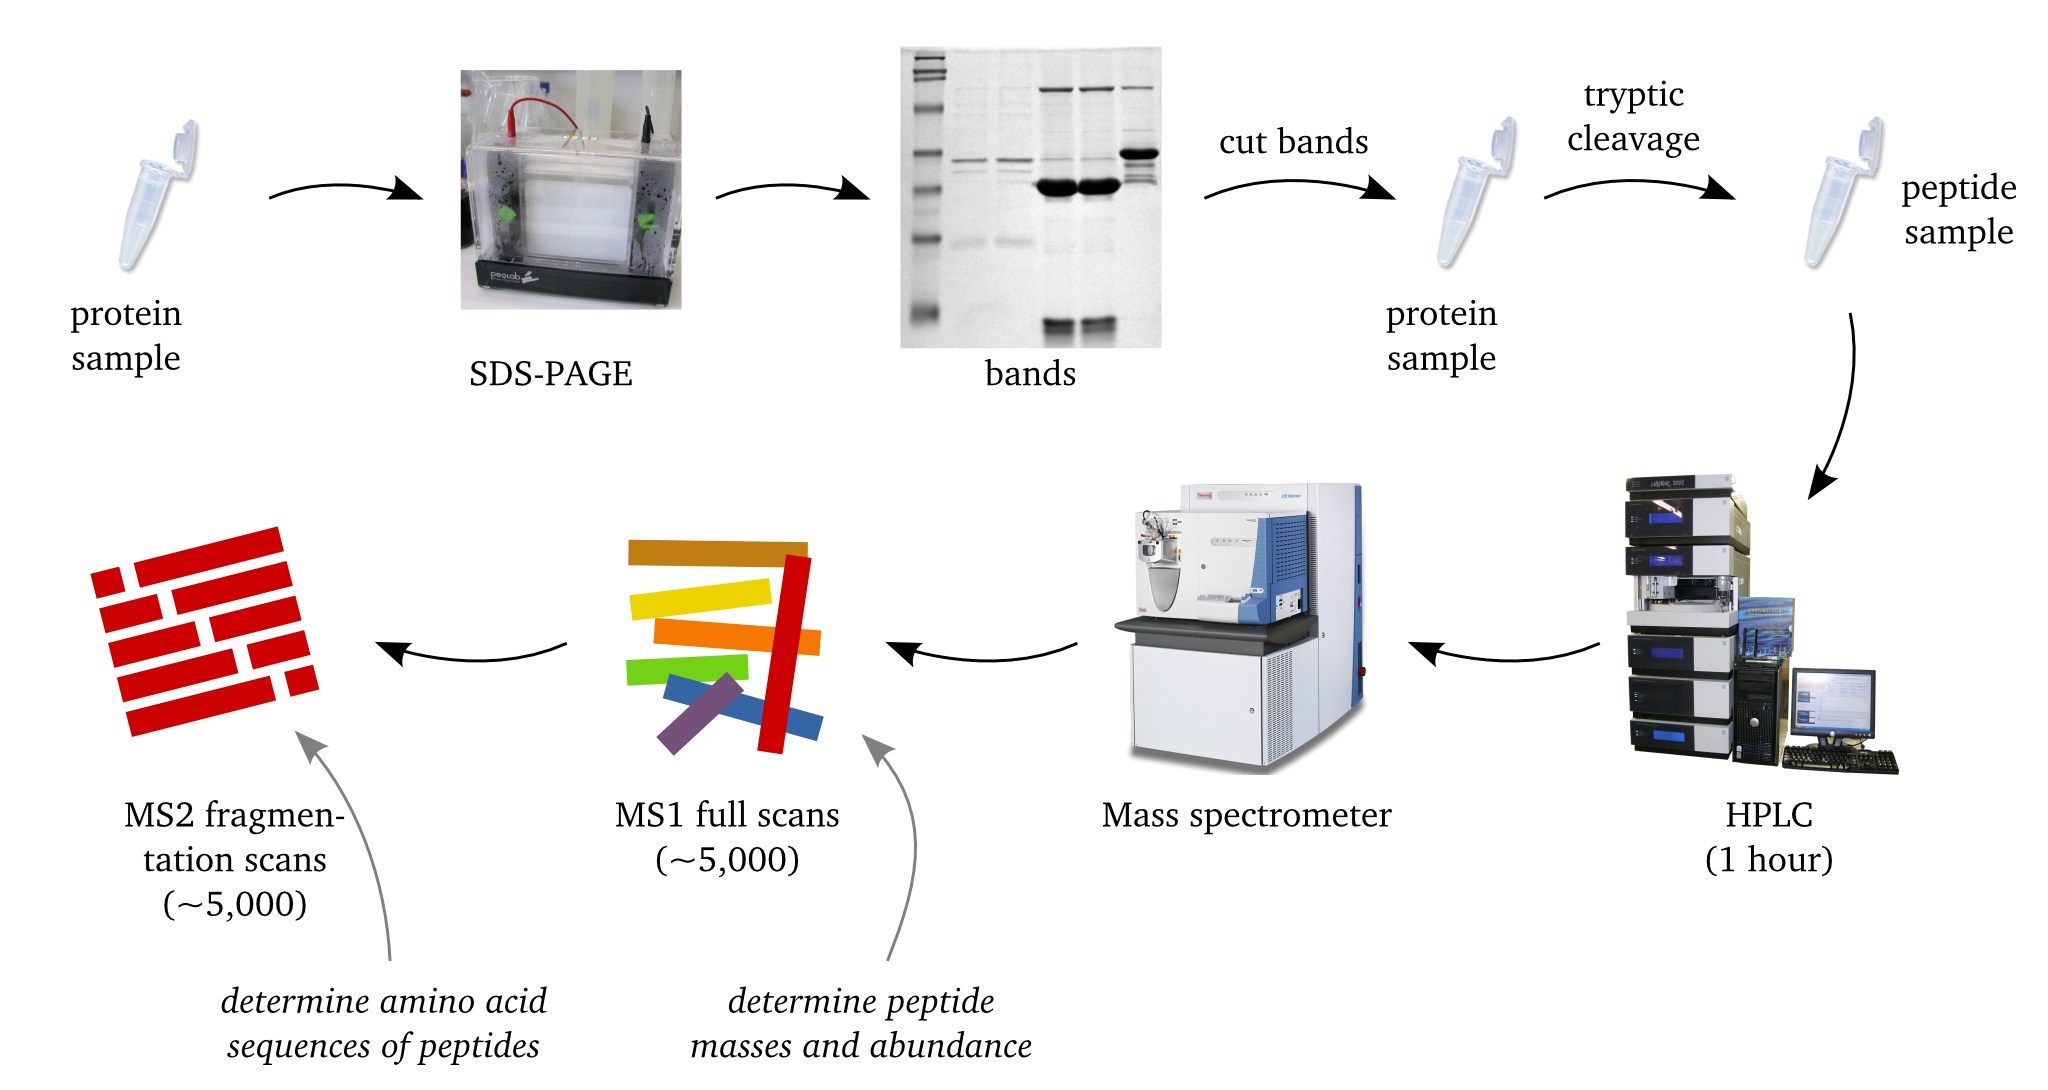
\includegraphics[width=\textwidth]{figures/Proteomics.jpg}
\caption{
{\bf Example of a mass spectrometry-based proteomics experiment workflow.} 
Protein samples are fractionated via SDS-PAGE and resulting bands are excised and
digested proteolytically. In order to further separate the complex mixture, 
the resulting peptides are loaded onto a HPLC column and subsequently eluted 
and injected into the mass spectrometer. Full scans and fragmentation scans
are recorded as peptide elution is in progress for a pre-defined amount of time.
}
\label{fig:proteomics-overview}
\end{figure}

% --------------------------------------------------------------
\subsection{Acquisition of mass spectrometric data}
% --------------------------------------------------------------

Using mass spectrometry, the mass of molecules cannot be directly determined
because mass analysis is always performed on ions of unknown charge, resulting
in a spectrum of intensity values for individual mass-to-charge ({\em m/z}) 
ratios.
When high {\em m/z} resolution is available, ion charges can be determined 
from a mass spectrum, and thus a deconvolution of {\em m/z} values to actual 
masses is possible.
Otherwise, the ambiguity introduced by the unknown charge state of detected
ions adds an additional level of complexity to data analysis.

% \subsubsection{Preprocessing of biological samples}

% \begin{SCtopfig}
% \centering
% 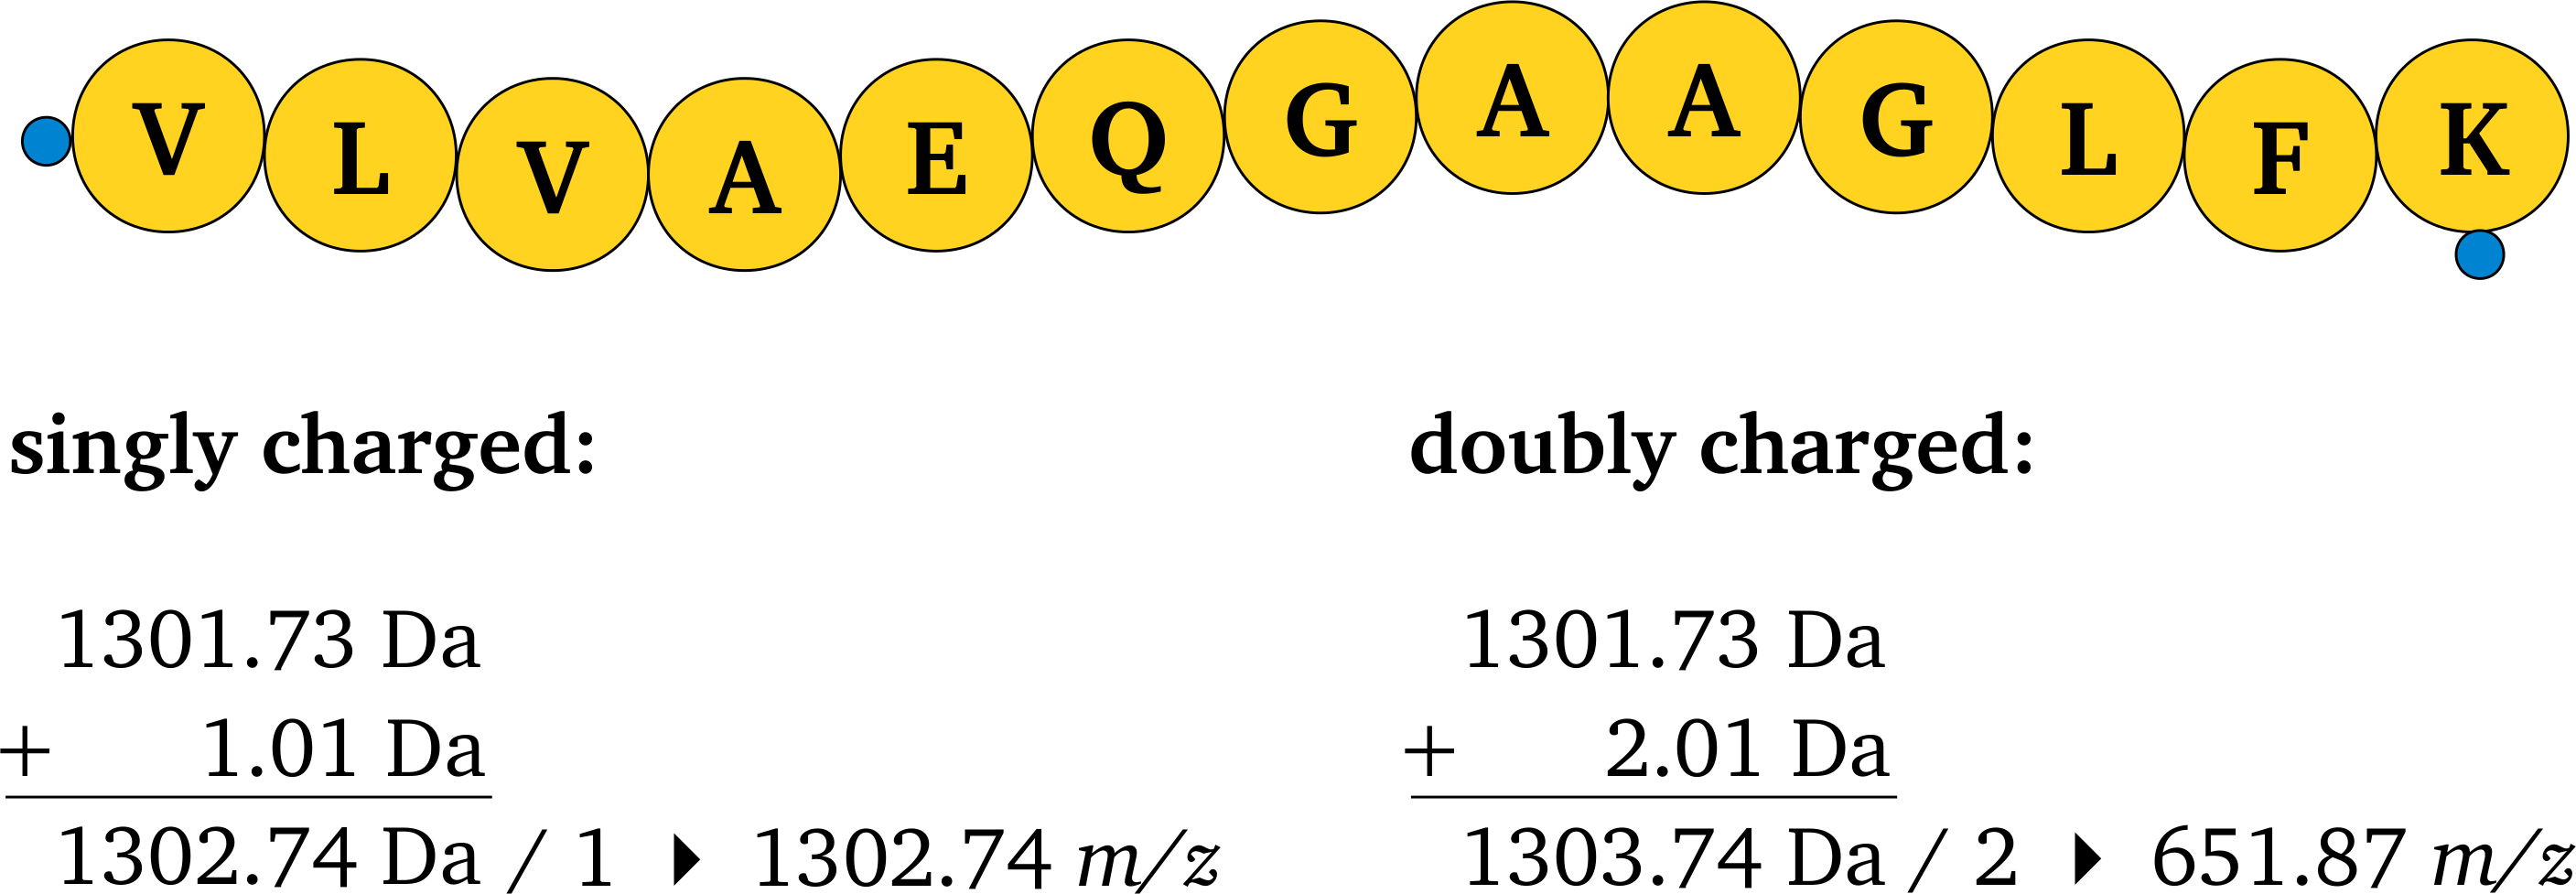
\includegraphics[width=0.7\textwidth]{figures/mz.jpg}
% \caption{
% {\bf Calculation of {\em m/z} values.}
% A single peptide may give rise to multiple {\em m/z} values in a mass spectrum,
%     depending on its charge. In this example, a singly and doubly protonated
%     peptide is shown.
% } 
% \label{fig:mz}
% \end{SCtopfig}

A common problem is that low abundant proteins may be missed in complex samples 
due to the fact that there are many more highly abundant proteins present.
To overcome these obstacles, several sample preprocessing steps, for example 
SDS-PAGE and liquid chromatography can be employed.
Although mass spectrometric analysis of intact proteins has been successfully
reported \citep{Lee2002, Taylor2003}, such an approach is not feasible in 
general because the high mass of proteins cannot be accounted for with most
types of mass spectrometers.
In order to break proteins up into small, mass spectrometry-compatible peptides, 
proteolytic enzymes are used.
Among the various choices of possible enzymes, Trypsin has become very popular
because it results in short peptides with a basic residue at the C-terminus
\citep{Olsen2004}.
% Trypsin cleaves specifically at the C-terminal side of Lysine and Arginine 
% residues, given that no Proline residue is located at the other side of the 
% cleavage site.
Alternative enzymes such as Asp-N and Glu-C are sometimes used to generate
complementing peptides which overlap with the tryptic peptides in order to 
increase sequence coverage of peptide identifications \citep{Steen2004}.
% Although Trypsin, Asp-N and Glu-C are very sequence-specific, the possibility 
% of missed cleavage sites must be taken into account during data analysis.

% \paragraph{Liquid chromatography}
% 
% In addition to fractionation via SDS-PAGE, liquid chromatography (LC) provides 
% a second dimension of separation, usually at the peptide level.
% For the experiments covered in this thesis, a reverse phase liquid 
% chromatography (RPLC) system has been employed.
% In this setup, peptides elute according to their hydrophobicity.

\paragraph{Ionization of molecules.}

In order to make molecules suitable for mass spectrometric analysis, 
the analyte must be ionized and transferred to the gaseous phase.
Among many available options, the two most widely used methods for this 
task are (1) matrix-assisted laser desorption/ionization (MALDI) for solid 
analytes, and (2) electrospray ionization (ESI) for liquid samples.
% MALDI
In the MALDI approach \citep{Karas1988}, the analyte is mixed with a 
matrix material and co-cristallized on a metal plate. 
A pulsing laser beam is used to excite the matrix and sublime several 
contained analyte molecules. 
Although initially, mostly matrix molecules get ionized by the laser
beam, charges are transferred to the analyte molecules while the
matrix/analyte cloud is moved towards the mass analyzer by an
electric field.
% ESI
ESI provides the advantage that it can be directly coupled to an
upstream LC system because it works with fluid samples \citep{Fenn1989}.
Here, the sample is pumped into a spray needle, either from the LC or via
direct injection. 
A high potential is applied between the entrance of the mass spectrometer and
the tip of the spray needle, resulting in electrostatic dispersion of the
effluent as it exits the needle tip.
The resulting charged droplet evaporates into smaller droplets until finally,
in the best case, only one analyte ion is contained in a single droplet.

\paragraph{Mass analysis and ion detection.}

Regardless of the ionization process, several options are available for
the most prominent part of a mass spectrometer, the mass analyzer.
% TOF
In the time-of-flight (TOF) mass analyzer \citep{Wolff1953}, equally charged 
ions are accelerated to the same kinetic energy, resulting in a velocity 
which is dependent on the {\em m/z} value of an ion, with lighter ions
moving faster than heavier ions.
The time required for the ion to hit the ion detector is measured and
then converted to the corresponding {\em m/z} value.
% Quadrupole
In the quadrupole mass analyzer \citep{Paul1956}, four parallel rods are 
used to create a radio frequency quadrupole field which can be controlled
in such a way that only ions of a specified mass-to-charge ratio can pass.
For the creation of a mass spectrum, the {\em m/z} range is traversed from
minimum to maximum and the passing ions are recorded.

% Ion traps

The third type of mass analyzer discussed in this thesis is the ion trap,
which is available in a couple of variants.
Common to all ion traps is that lower analyte amounts are required as
compared to quadrupole mass analyzers, because instead of scanning
the entire {\em m/z} range as the sample passes through the mass spectrometer 
and discarding all ions which do not match the current {\em m/z} value, 
ions are first trapped and collected in the ion trap and then ejected 
sequentially, traversing the entire {\em m/z} range.
In the three-dimensional quadrupole ion trap, ions are trapped in a space
confined by a ring electrode and two endcap electrodes.
The linear ion trap uses a two-dimensional field and provides for higher ion
storage capacity, resulting in an increased detection sensitivity.
The Fourier transform ion cyclotron resonance (FT-ICR) mass analyzer provides
for extremely high mass resolution which.
However, a strong magnetic field must be created and sustained, resulting
in high maintenance as the system needs to be constantly cooled with helium. 
The most recent development in this area, the Orbitrap, combines high mass 
accuracy with low maintenance requirements \citep{Hu2005}. 
A Thermo Scientific LTQ Orbitrap XL mass spectrometer has been used for the
acquisition of all mass spectrometric data used in this thesis.

Another aspect of ion traps is that fragmentation of previously selected,
specific precursor ions becomes possible.
This is a prerequisite for tandem mass spectrometry (MS/MS), or data dependent
acquisition.
Here, a pre-defined, fixed number of highly abundant precursor ions is selected
from every full scan, and subsequently subjected to fragmentation
in a process called {\em collision induced dissociation} (CID).
Here, peptides collide with an inert gas and subsequently break apart into 
N- and C-terminal fragments, thereby producing {\em b} ions and {\em y} ions, 
respectively. 
Depending on the actual fragmentation site within the peptide bond,
alternative fragment ions may result: {\em a} and {\em c} ions for N-terminal
fragments, {\em x} and {\em z} ions for C-terminal fragments.

% \subsection{Mass spectra}

Recorded mass spectra are stored as vendor-specific files which contain meta 
information which describes the acquired data as well as the raw peak data.
In order to unify the exchange of mass spectrometers raw data, the mzML file 
format has been devised by the HUPO Proteomics Standards Initiative
\citep{Deutsch2008}.
Apart from the file format details, several different scan types can be
acquired, each of which contains different information.

\paragraph{Full scans (MS).}

Full scans provide an overview over the peptides which are present in the
mass spectrometer at a given time (see Fig.~\ref{fig:full-scan}).
The \mz~values of all intact peptides are reported.
However, the absence of a precursor peak does not necessarily indicate the
absence of the corresponding peptide in the sample, because detection of
an ion may fail for various reasons.
Following a full scan, one or more highly abundant precursors are usually
selected for further analysis.

\begin{figure}
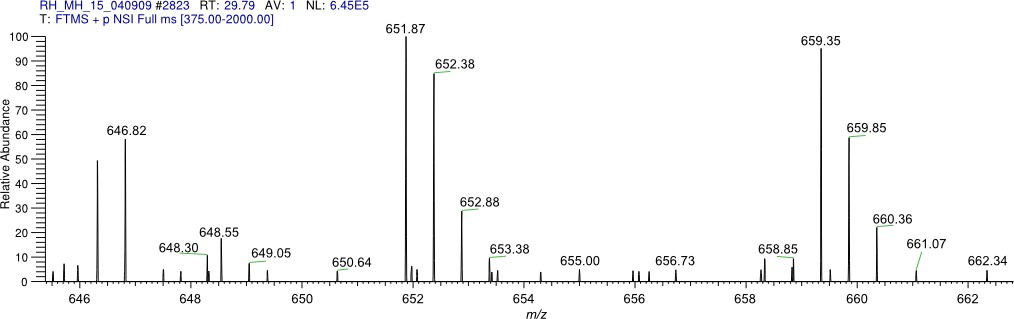
\includegraphics[width=\textwidth]{figures/ms1-scan.jpg}
\caption{
{\bf Zoomed view of a full scan.}
Isotope envelopes of doubly charged peptides, consisting of precursor
peaks with a \mz~difference of $\sim0.5$ are visible,
}
\label{fig:full-scan}
\end{figure}

\paragraph{Fragmentation scans (MS/MS).}

The scans resulting from collision-induced dissociation are called 
fragmentation scans, or tandem MS (MS/MS) scans (see Fig.~\ref{fig:fragmentation-scan}).
From the observed fragment ions, {\em mass ladders} can be constructed which
represent the amino acid sequence of the selected peptide (see Fig.~\ref{fig:fragmentation-scan-b-y}). 
When fragmentation peaks are missing, the exact sequence of the peptide may not
become clear from a single mass ladder.
However, a combination of multiple mass ladders can resolve such ambiguities.

\begin{figure}
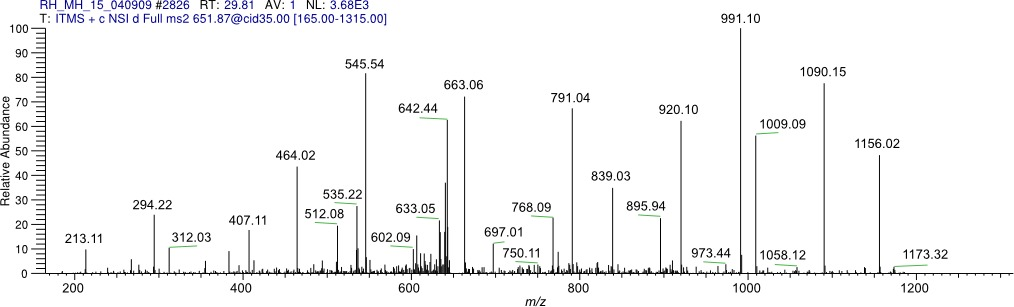
\includegraphics[width=\textwidth]{figures/ms2-scan.jpg}
\caption{
{\bf Example of a fragmentation scan.} 
The 651.87 \mz~precursor peak shown in Fig.~\ref{fig:full-scan} has been
subjected to collision-induced dissociation.
Resulting fragment ions are recorded in the fragmentation scan.
}
\label{fig:fragmentation-scan}
\end{figure}

\begin{figure}
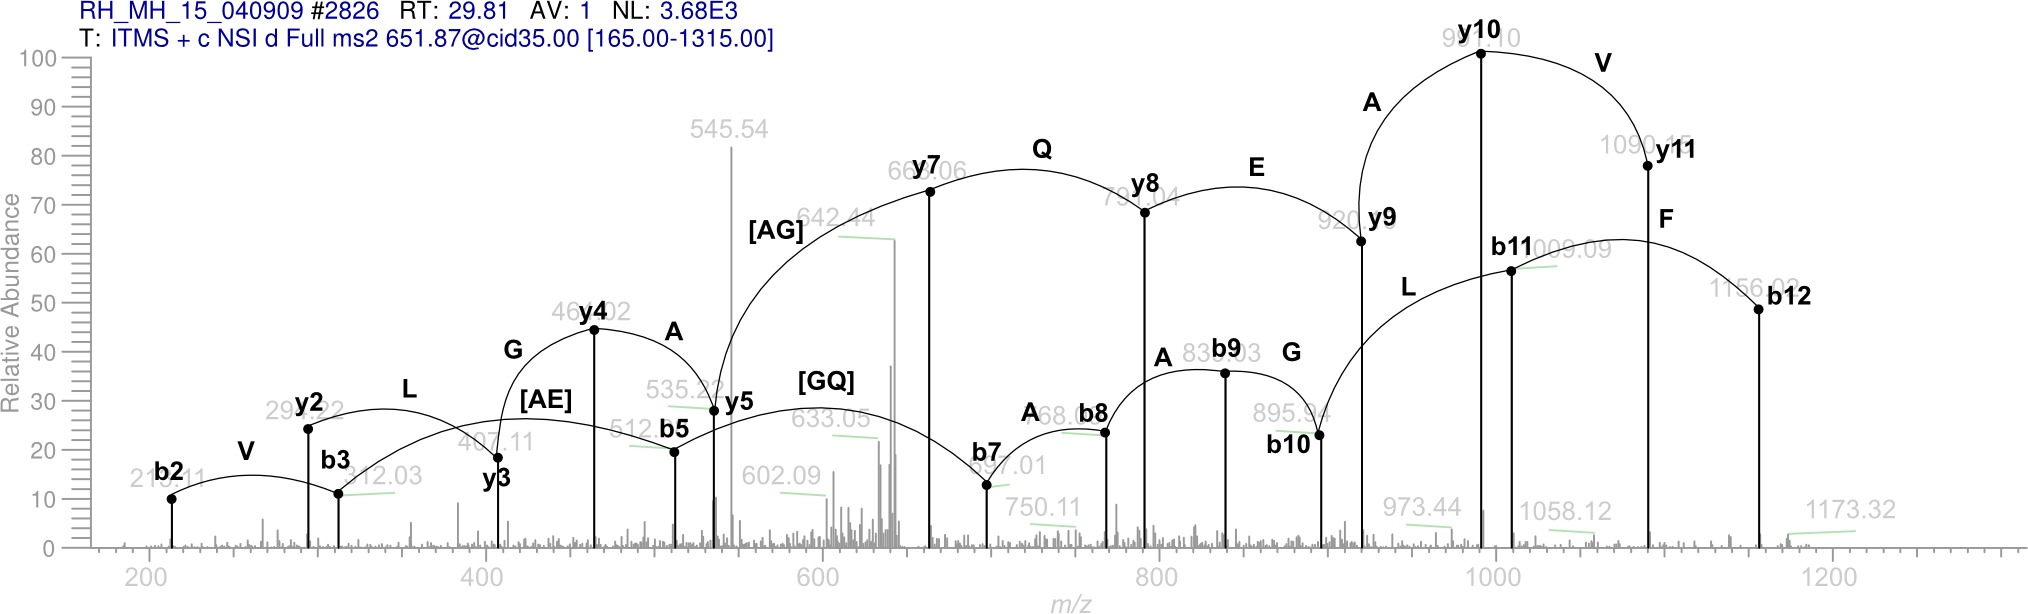
\includegraphics[width=\textwidth]{figures/ms2-scan-b-y-1.jpg}
\caption{
{\bf The MS/MS scan depicted in Fig.~\ref{fig:fragmentation-scan} with {\em b} and 
{\em y} ion series mass ladders superimposed.} 
The \mz~differences of fragmentation peaks reflect the masses of individual amino
acids or short amino acid oligomers.
}
\label{fig:fragmentation-scan-b-y}
\end{figure}


% --------------------------------------------------------------
\subsection{Identification of peptides and proteins}
% --------------------------------------------------------------

Evaluation of the acquired mass spectrometric data is a process with a multitude
of possible options.
Usually, the decisions made during sample preparation and data acquisition are
reflected in the data analysis: If proteins were separated via SDS-PAGE, the
resulting order of proteins via their mass can be used to verify or falsify 
identifications.
Likewise, if liquid chromatography is employed, the retention time at which
peptides have been identified can be used for plausibility checks.

Sequence databases, including genome and protein sequences, play an important
role in MS/MS data evaluation because they greatly confine the search space
for peptide identification from MS/MS spectra.
However, care must be taken if these databases are not comprehensive, because
the search space defined by incomplete sequence databases might be too small
to provide for proper identification.


% \subsubsection{Identification}

Several possibilities have been established to identify peptides present
in the sample. 
Usually, only a fraction of all peptides present in a sample can be 
identified for various reasons.
Firstly, peptides stemming from low abundant protein may be missed because 
they result in low precursor peaks which are generally less favored, and
therefore harded to detect, when compared to high peaks that can be clearly
distinguished from noise peaks.
Another problem arises when highly complex samples are used and the
high number of peptides outnumbers the number of scan events in the
mass spectrometric run.
Also, highly abundant peptides are prone to be identified repeatedly,
thus decreasing the identification chances of low abundant peptides.
Finally, the differing physicochemical properties of all peptides
lead to the effect that only a subset of the sample can be ionized and
fragmented in such a way that identification is possible.

\paragraph{Peptide mass fingerprinting.}

Peptide mass fingerprinting is a protein identification method which was
simultaneously developed by several groups in 2003 
\citep{Henzel1993,James1993,Mann1993,Pappin1993a,Yates1993}.
In this method, the observation of several intact peptide precursor masses
(the peptide mass fingerprint) is used to identify the protein which was 
present in the sample.
Peptides are determined {\em in silico} prior to the search from a protein
database and their masses are subsequently matched to the observed precursor
peaks.
Accoring to \citet{Mann1993}, four to six proteolytic peptides measured
at a mass accuracy between 100 and 1,000 ppm are usually sufficient to
characterize a protein.
The acquisition and interpretation of fragmentation is scans is not required, 
however the method has the disadvantage that only samples containing a single 
protein can be analyzed and complex protein mixtures cannot be used.

\paragraph{Database search.}

\begin{figure}
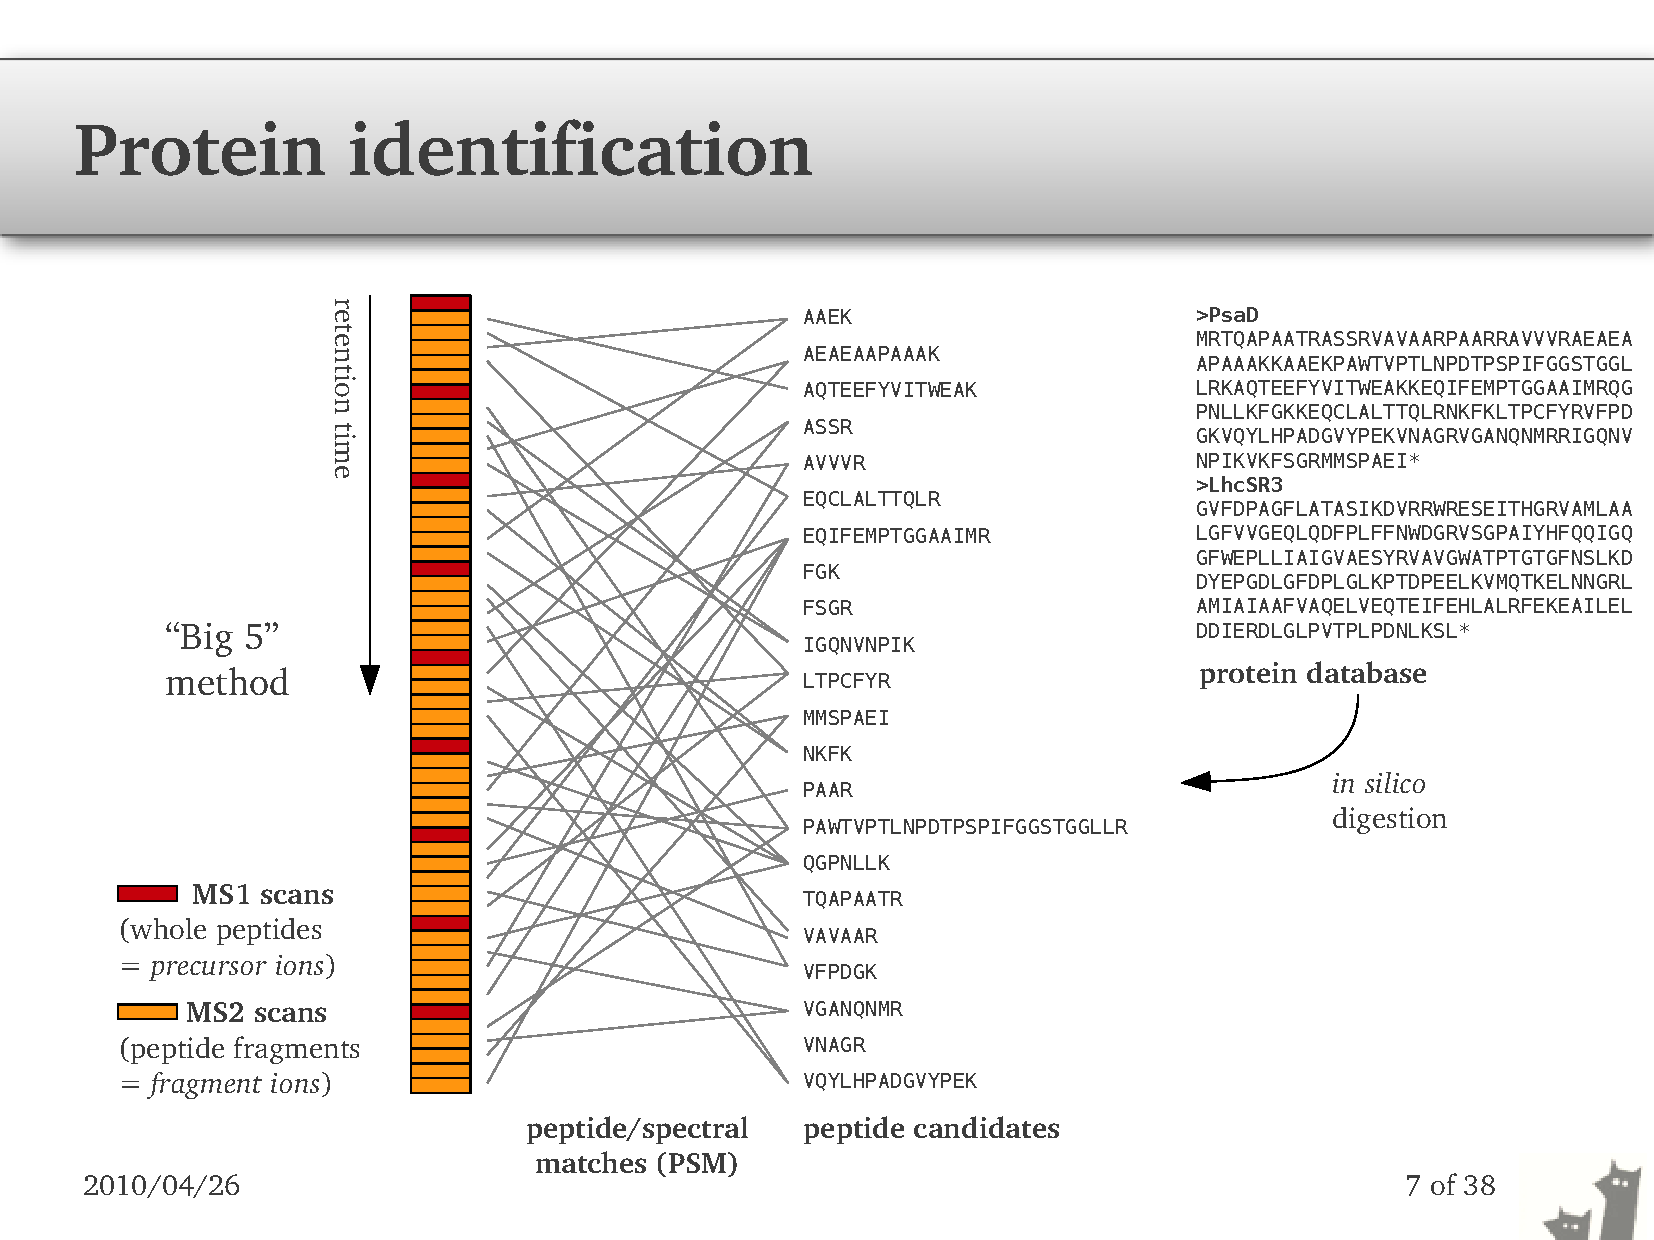
\includegraphics[width=\textwidth]{figures/psm.jpg}
\caption{
{\bf The peptide/spectral matching strategy implemented by database search 
programs.} 
Protein sequences are digested {\em in silico}, mimicking the {\em in vitro}
enzymatic digestion of proteins. 
The resulting peptides are then matched to recorded fragmentation scans,
usually resulting in multiple matches per spectrum.
Further ranking and filtering steps are employed to determine the presumably
correct identification.
}
\label{fig:psm}
\end{figure}

One year after the advent of the peptide mass fingerprint approach, a novel
method for the identification of peptides was developed by \citet{Eng1994}.
In their study, \citeauthor{Eng1994} introduced SEQUEST, an algorithm which
takes fragmentation scans and a protein sequence database as input files.
From the protein sequences, {\em in silico} digested peptides are determined
and their theoretical fragmentation scans predicted.
Finally, using the precursor mass as a first filtering criterion, all
theoretical and measured fragmentation scans are compared via cross-correlation
and the resulting matches are scored and ranked.
Subsequently, the best matching peptide is regarded as the correct 
identification of the corresponding fragmentation scan, given that there is
no different, competing identification with a similarly good score (see 
Fig.~\ref{fig:psm}).
This prerequisite for the correctness of peptide identifications highlights
a drawback of the method: as for peptide mass fingerprinting, the peptide
identification completely depends on the protein sequence database used.
Sequences which are not covered by the database are not tested and therefore
cannot weaken the identification distinctness of a particular peptide/spectral 
match (PSM).
In the recent years, several new database search programs have become 
available, including MASCOT \citep{Perkins1999}, X! Tandem \citep{Craig2004},
OMSSA \citep{Geer2004}, and MyriMatch \citep{Tabb2007}.

\paragraph{Statistical assessment of peptide/spectral matches.} 

Initially, individual peptide/spectral matches had to be validated manually,
and consensus score thresholds could be used as a rough estimate to distinguish
incorrect from correct peptide identifications.
With the advances in mass spectrometry leading towards high-throughput analyses,
such an approach was no more feasible and a method for the assessment of
the statistical significance of peptide/spectral matches was required.
Two methods were developed for this purpose: 
In \citeyear{Keller2002}, \citeauthor{Keller2002}~proposed an algorithm which
assumes the score distribution from a set of 
peptide/spectral matches to be composed of two distinct distributions,
one for incorrect, and one for correct assignments. 
The algorithm presented in their study \citep{Keller2002}, PeptideProphet,
attempts to disentangle these distributions and separate false from correct
identifications.
An alternative approach which is very flexible and easy to implement was
proposed five years later by \citeauthor{Elias2007}.
In their paper, the authors proposed a target/decoy search strategy to 
facilitate posterior probability estimation of the complete list of
peptide/spectral matches resulting from a database search \citep{Elias2007}.
To achieve this, the input protein database is complemented with an equally 
sized {\em decoy database} which contains sequences derived from the original
database entries by reversing or shuffling the amino acid sequence.
To the database search program, peptides from both target and decoy sequences 
appear as equal candidates to explain fragmentation scans.
From the resulting of list of assignments, a score threshold can be determined
in such a way that a user-defined estimated false discovery rate (FDR) is
achieved in regard to the complete set of identifications.
In practice, the score threshold is determined by traversing the entire PSM 
list, starting from the best-scoring assignment and counting the number
of true (target) and false positive (decoy) hits.
Based on these numbers, \citeauthor{Elias2007} estimate the FDR as

\begin{equation}
\text{FDR} = \frac{2 \cdot n_{\text{decoys}}}{n_{\text{targets}} + n_{\text{decoys}}}.
\end{equation}

\citeauthor{Kall2008a} propose an alternative FDR estimation 
\citep{Kall2008a}:

\begin{equation}
\text{FDR} = \frac{n_{\text{decoys}}}{n_{\text{targets}}}.
\end{equation}

Regardless of the actual estimation, the target/decoy approach is based on 
the following assumptions \citep{Elias2007}: (1) proteolytic peptides inferred 
from the target and decoy databases do not overlap, and (2) false positive 
identifications from both databases are equally likely.
These requirements have implications for the creation of the decoy sequences
and as a consequence, there is an upper database size limit for which the 
target/decoy approach is feasible.

\paragraph{{\em De novo} sequencing.}

For the interpretation of fragmentation scans, {\em de novo} sequencing is
a highly unbiased method.
Here, the mass ladders recorded in a fragmentation scan are reconstructed
and a list of full peptide sequence candidates is returned as a result.
Because the assignment of peptides to fragmentation spectra does not rely
on a sequence database, the identifications are unbiased and especially
useful for organisms with unsequenced genomes or incomplete genome sequences.
Due to the inherent ambiguities regarding the interpretation of fragmentation
peaks and their assignment to {\em b} or {\em y} ion mass ladders, and the 
problem of interfering noise peaks, interpretation is difficult and 
high-resolution spectra are usually required to achieve correct results.
In addition, the speed of such algorithms is generally very low because the
search space is only confined by the proteolytic enzyme which was used
for protein digestion and apart from that, all possible amino acid sequences
must be taken into account.
Available {\em de novo} sequencing programs include Lutefisk 
\citep{Johnson2002}, PEAKS \citep{Ma2003} and PepNovo \citep{Frank2005}.

A common problem with {\em de novo} sequencing is that the resulting peptides
are generally not completely correct across the entire amino acid sequence, 
and an automated method to validate peptides and use the resulting validated 
peptides in a downstream analysis is not readily available. 
Therefore, {\em de novo} sequencing is often used as a complementing method 
which is used in special cases and requires manual verification.
A hybrid approach combining {\em de novo} sequencing and database search
is implemented by sequence tag search algorithms such as InsPecT 
\citep{Tanner2005} or ByOnic \citep{Bern2007}.
Here, short sequence tags, consisting of a short amino acid sequence and the
masses of the N- and C-terminal fragments are extracted from the fragmentation 
spectrum.
The subsequent database search is restricted to the peptides which match
the extracted sequence tag, thereby increasing search speed.


\subsection{Quantitation of peptides and proteins}

In addition to determining which peptides, and therefore proteins, are 
contained in a sample, it is often of interest to determine the abundance
of proteins in samples from different conditions \citep{Schulze2010}.
Using this information, the effect of various influences, such as environmental 
stress or periodic environmental changes such as the light-dark cycle,
can be elucidated.
Generally, two samples are compared in one experiment and in most approaches, 
quantitation results are relative, indicating up-regulation, down-regulation 
or unchanged abundances for various proteins.
If a standard of known amount is spiked into the sample and quantified alongside
the proteins of interest, these relative results can typically be promoted to 
absolute quantitation results.

\paragraph{Chemical labeling.}

Chemical labeling methods introduce a label into the peptides from one of the 
samples via a chemical reaction. 
The {\em isotope-coded affinity tag} method (ICAT) 
uses two affinity tags {\em d0} and {\em d8} which bind to cysteine residues
and introduce a mass shift of 0 and 8 Da, respectively \citep{Gygi1999}.
The mass shift of 8 Da can be observed in the full scans and the area under
the respective precursor ion isotope envelopes can be used to estimate
the ratio of peptide abundance in both samples.
However, because the method is restricted to mass spectrometry-compatible 
peptides which contain a cysteine residue, ICAT yields comparably low proteome
coverage.

The {\em isobaric tag for relative and absolute quantitation} method (iTRAQ)
follows a similar approach by introducing isobaric tags into the peptides in
different samples \citep{Ross2004} at the stage of enzymatic digestion.
However, the N-terminus of peptides is labeled, resulting in increased proteome
coverage.
Each iTRAQ tag consists of a reporter group and a balance group, which together 
result in a mass shift of 145 Da. 
However, several distinct tags are available and possible reporter group masses 
include 114 Da, 115 Da, 116 Da, and 117 Da, thus enabling the simultaneous 
analysis of more than two samples (an iTRAQ variant with 8 different tags is also
available).
The isobaric tags result in the effect that equal peptides from different 
samples appear at the same {\em m/z} value in the full scan.
During fragmentation, the reporter groups get separated from the peptide, 
resulting in distinct reporter peaks in the fragmentation scan, allowing
for subsequent quantitation of peptides identified via tandem mass spectrometry.
In comparison to the ICAT method, peptide quantitation is only performed in 
fragmentation scans and therefore the amount of sampled quantitation ratios 
per peptide is usually low.

\paragraph{Metabolic labeling.}

As an alternative to chemical labeling, metabolic labeling can be used for
peptide and protein quantitation in organisms which can be forced to incorporate
an isotopically labeled amino acid or a stable isotope of a certain chemical 
element.
In this approach, the label is introduced via the metabolism of an organism.
In the {\em stable isotope labeling with amino acids in cell culture} method
(SILAC), strains are required which are not able to synthesize certain amino
acids such as Arginine or Lysine \citep{Ong2002}.
For \cre, the Arginine-auxotrophic strain CC424 is available which
must be supplied with Arginine to survive.
The fact that $^{13}$C-labeled Arginine exposes the same physicochemical 
properties as the natural $^{12}$C Arginine and thus the organism is 
oblivious to the isotopically labeled variant can be used to create 
unlabeled and labeled samples which can later be mixed and measured in a 
single MS/MS experiment.
Using tryptic peptides and a $^{13}$C-Arg label, a mass shift of 6 Da is 
typically introduced for each peptide because one Arginine amino acid 
contains six carbon atoms.
Due to the physicochemical equality of sister peptides in the mixed sample,
equal peptides from both conditions can be expected to co-elute and therefore
appear next to each other in several full scans. 
From peptide identifcations in nearby fragmentation scans, the identity of
sister peptide precursor peaks can be assumed and subsequently, the peptide
can be quantified.
In the case of $^{13}$C-Arg labeling, only 50\% of all tryptic peptides can
be expected to be suitable for quantitation, because trypsin cleaves C-terminal
of Arginine and Lysine residues, resulting in roughly half of all tryptic 
peptides containing no Arginine at all.
However, different variations are possible, for example, $^{13}$C-Arg/Lys 
labeling can be used, although this requires a strain which is both Arginine
and Lysine-auxotrophic.

\paragraph{Label-free quantitation.}

In the recent years, label-free quantitation methods have been developed and
constantly refined.
In these approaches, no labels are required and measurements of two or 
more samples are cross-correlated to determine relative peptide and protein
amounts in the respective conditions.
Spectral counting is a coarse and simple way of assessing protein ratios by
comparing the number of scans a peptide, and therefore protein, was identified
in across the samples \citep{Old2005}.
Given that a minimum number of peptide/spectrum matches could be obtained from
each sample, a rough estimation of the protein ratio can be performed.
However, it must be taken into account that the number of triggered and
subsequently identified scans for a peptide depends on many factors.
In addition, if a dynamic exclusion filter is employed during the measurement 
to disable re-triggering of the same highly abundant precursor {\em m/z} value 
for a certain time (typically 90 seconds), this effect must be taken into 
account when peptide abundance is inferred from the number of scans a peptide
has been identified in.

More precise results can be obtained using tools which operate on full scans
to determine peptide ratios \citep{Mueller2007, Park2008}.
In these approaches, peptide precursor peaks in different runs are correlated 
without the requirement of explicit MS/MS identification within the same run.
This is achieved by establishing a database of {\em accurate mass/time tags} 
(AMT tags) which describe full scan features (individual peptides) by means
of accurate mass and retention time.
This repository can than be used to ascertain the identity of specific precursor
peaks which have not been subsequently triggered for collision-induced 
dissociation but have been identified in a different run at the same retention 
time.
In order to accomodate for variations in the LC elution, all involved runs
must be aligned in such a way that equal peptide elute at equal retention times.
While retention time alignment is a complex and inherently ambiguous process
\citep{Fischer2006}, label-free quantitation can be regarded as a very powerful
quantitation strategy because it provides comprehensive results and recorded 
mass spectrometric data can regularly be re-evaluated using an updated AMT tag 
database, potentially yielding more results as the proteome coverage in
the database becomes saturated.


\section{Proteogenomics}
\label{proteogenomics}

Genome sequence databases are a prerequisite for the prediction of protein 
databases, and full genome sequences for more than 180 species are available
\citep{Yates2009}.
The annotation of genomic sequences remains a challenge, especially in
eukaryotic genomes, where protein coding sequences are often interrupted by
introns.
% bad quality
Published gene models for organisms are subject to frequent changes and updates
following manual inspection or novel strategies for gene model prediction.
In the {\em A. thaliana} gene models, more than 1000 genes needed corrections
and over 250 novel genes were added with the release of version 9 of the
Arabidopsis Information Resource (TAIR, \cite{Huala2001}).
In the case of {\em C. elegans}, manual inspection of the predicted gene models
revealed that 50\% of all genes required corrections \citep{Reboul2003}.
Likewise, a manual inspection of human gene models resulted in the 
identification of additional exons for 80\% of all gene models 
\citep{Pennisi2007}.
These reports show that correct genome annotation is a strongly debated
topic and therefore a vital area of research, especially because it forms
the foundation of many post-genomic applications.

% EST support
Various strategies have been proposed to identify protein coding genes in
genomic sequences using expressed sequence tags (EST) libraries, 
including the UCSC KG II \citep{Karolchik2003}, ENSEMBL \citep{Hubbard2005} 
and NCBI Gnomon annotation pipelines \citep{Maglott2005}.
In these approaches, genes are identified by mapping known cDNA tags to the
genomic DNA sequence.
Consequently, high cDNA coverage is required to achieve comprehensive
genome annotation and therefore, low expressed transcripts pose a challenge.
% comparative
When cDNA information is unavailable, information from closely related
species can also be used for genome annotation.
Several software tools which implement this approach are available,
including TWINSCAN \citep{Korf2001}, SGP 2 \citep{Parra2003}, and 
SLAM \citep{Cawley2003}.

As an alternative to cDNA and conservation supported genome annotation,
{\em ab initio} genome annotation can be used for species for which no
or only little cDNA evidence is available and no closely related annotated
species exists.
In this approach, statistical calculations are performed on the genomic
DNA sequence, assessing various properties such as codon usage and splice 
site consensus sequences.
This approach allows for the initial annotation of novel genomic DNA 
sequences.
Programs using this approach include GENESCAN \citep{Burge1997}, 
GENEID \citep{Parra2000}, and AUGUSTUS \citep{Stanke2004, Stanke2006}.
As a result of recent developments, initially unbiased {\em ab initio} 
genome annotations can be supplemented with extrinsic information as it 
becomes available \citep{Stanke2008}, thus refining the genome annotation.
This multilateral strategy seems to be indispensable for eukaryotic genomes
where gene prediction is complicated by long introns and alternative splicing
\citep{Brent2004}.

\paragraph{Proteogenomic genome annotation.}

From the mass spectrometry perspective, the recent advances represent a
promising perspective: In addition to EST evidence and conserved genes in
related species, peptides identified in MS/MS scans can be used to support
genome annotation.
This approach has several advantages. Firstly, peptides that have been observed
in fragmentation scans can be used to differentiate pseudogenes from coding 
genes. 
Second, observed peptides can be used to ascertain that gene transcripts
are not degraded but actually expressed as proteins.
In addition, identified peptides automatically determine the coding frame
for a certain genomic region and elucidate the location of introns in a gene.
An additional benefit of MS/MS-assisted genome annotation is that scans recorded
in many experiments for various experimental purposes can be used to provide
extrinsic peptide hints to the gene model prediction program and measurements 
with the specific aim of generating peptide hints are usually not required.

The central challenge in generating peptide hints is to correctly identify
peptides from fragmentation spectra in a way that is unbiased towards existing,
potentially misleading gene models. 
In addition, the identification of spliced peptides is especially helpful
because these peptides can be used to establish a connection between two
coding regions in the genome.
A simple solution could be implemented by using the entire six frame translation
of a genome as a protein database and matching fragmentation spectra against
it.
However, the assessment of the statistical significance of these hits is 
difficult, given that the amount of false peptides in the six frame translation
is unknown and at least 83\% because for a certain genomic region, at most
of six reading frames can be expected to be protein-coding.
In addition, this method does not yield spliced peptides which are highly
interesting for the annotation of complex eukaryotic genomes.

% \subsection{The exon splice graph approach}

In \citeyear{Tanner2007}, \citeauthor{Tanner2007} proposed an approach to
perform identification of spliced peptides within a genomic DNA sequence 
\citep{Tanner2007}.
The method proposed in the study uses splice site prediction and compiles
a compact representation of all putative exons and splice junctions in a 
graph.
A specialized database search tool is then used to match fragmentation spectra
to peptides contained in the exon splice graph.
Using this method, \citeauthor{Castellana2008} were able to revise the 
annotation of {\em A. thaliana} by correcting 695 genes and identifying
778 novel genes.

\paragraph{The Genomic Peptide Finder.}

\label{section:gpf}

The Genomic Peptide Finder (GPF), originally devised by \citeauthor{Allmer2004} 
in \citeyear{Allmer2004}, follows a different strategy for the use of 
{\em de novo} predicted amino acid sequences \citep{Allmer2004}.
Instead of matching short sequence tags to gene model proteins, GPF uses the
six frame translation of a genomic DNA sequence as a matching target.
From a given {\em de novo} sequenced peptide, all sequence tags of a 
user-defined size are extracted and each of the sequence tags is located
within the six frame translation.
From the resulting locations, the deduction of candidate peptides is attempted,
each of which could be a possible explanation of the fragmention scan the
{\em de novo} sequenced peptide originated from.
All deduced candidate peptides fulfill the following criteria:

\begin{itemize}
\item a short sequence tag (typically three to five amino acids) has been 
correctly predicted via {\em de novo} sequencing 
\item the position of the sequence tag within the peptide, as defined by
either the N- or C-terminal fragment mass, is correct within the limits 
defined by the fragment scan mass accuracy (typically 700 ppm for an ion trap)
\item the total mass of the peptide matches the observed precursor mass
within the range defined by the full scan mass accuracy (typically 5 ppm for 
the Orbitrap)
\end{itemize}

In addition to unspliced candidate peptides, the deduction of spliced candidate
peptides is attempted by considering a user-defined maximum intron length.
The resulting peptides may then be used to verify or falsify existing gene 
models, as shown in a subsequent publication where GPF was used to confirm 
2174 gene model peptides and further identify 448 novel peptides, including 98 
spliced peptides \citep{Allmer2006}.
The manual inspection of the identified peptides lead to the identification
of novel gene models, the improvement of existing gene models as well as 
hints for alternative splicing.

% --------------------------------------------------------------
\section{Software solutions for MS/MS data evaluation}
% --------------------------------------------------------------

Although manual interpretation of mass spectrometric data, including
peptide and protein identification and quantitation, is possible and was
the only possibility in the beginning of mass spectrometric research, dedicated 
software is essential today in order to deal with the massive amounts of data
generated in high-throughput experiments.
Despite the numerous applicable techniques for the reduction of mass spectrum
complexity, interpretation of mass spectra is still hampered by a certain
level of ambiguity introduced by several factors, including multiply charged, 
overlapping ions and missing fragment ions in MS/MS scans.
In the face of high complexity, it is therefore vital to define clear
rules and solid models for the interpretation of mass spectra.
Given these rules and models, expert interpretation and computational 
analysis both have their advantages and disadvantages.
While an algorithm executed by a computer is typically strictly deterministic 
and less susceptible to external influences, and produces the same results
when repeated on the same input data, a human expert is capable of detecting 
situations in which previously made assumptions must be challenged and 
subsequently, models must be adjusted to reflect the changed preconditions.

Regardless of these differences, it is obvious that for large-scale data
evaluation, it is more efficient to invest human field-specific expertise and
software engineering skills to create an automated algorithm which subsequently
performs the data interpretation.
This way, it can be ensured that the interpretation of mass spectrometric data 
is consistent across one version of the software and in the case of false
assumptions or ill-designed models, a uniform re-interpretation of previously
acquired data is possible in a short time.
Software solutions therefore play a key role in today's mass spectrometric 
experiments.

Concerning the evaluation of mass spectrometric data, SEQUEST was the first
program to implement protein database-driven annotation of MS/MS spectra 
\citep{Eng1994}.
It has inspired a large number of alternative solutions for this problem,
including commercial and freely available software.
Likewise, various commercial and freely available tools for peptide and
protein quantitation exist, comprising the entire range of chemical and 
metabolical labeling as well as label-free techniques \citep{Vaudel2010}.

\paragraph{MS/MS data processing infrastructure.}

Apart from the actual software tools which perform mass spectrometric data 
interpretation, additional infrastructure is required to enable user-friendly 
control of these programs.
Most importantly, such an infrastructure must be able to handle the 
high-troughput capabilities of today's LC-MS/MS setups.
The Trans-Proteomic Pipeline (TPP) was the first MS/MS-specific data evaluation 
platform to be released (\cite{Keller2005}).
It allows users to run various programs on MS/MS data files.
It is platform-independent and supports a large selection of commercial and
free software.
% However, TPP requires the installation of an Apache web server for the purpose
% of providing a web browser-based graphical user interface (GUI).
% While the graphical user interaction is helpful for users, the required Apache 
% web server presents a non-negligible security risk because it potentially renders 
% the user's computer accessible and exploitable from the Internet when it can be 
% expected that most users won't be aware of this issue and will therefore not 
% be able to regularly apply security patches. 
% This issue is especially precarious on Windows and Mac OS X which do not 
% natively provide centralized, automatic software updating.
The web server-based approach implemented by TPP lends itself to a centralized
setup where a central server performs the actual data processing and can
be controlled by external clients via the web browser.

The OpenMS Proteomics Pipeline (TOPP) is another recently released software 
system for the evaluation of MS/MS data \citep{Kohlbacher2007}.
TOPP is based on the OpenMS C++ library which provides misceallaneous mass 
spectrometry-related functionality to software developers as a programming 
library.
Aside from providing a substantial body of software tools on the command-line 
interface (CLI), TOPP provides a GUI to these tools which can be used to
construct and execute MS/MS data evaluation pipelines.
In comparison to the web server-based approach followed by TPP, TOPP implements
a more distributed approach because the installation of a web server is not
required and a platform-independent GUI is provided via the Qt framework.

Systems biology approaches in which model organisms are characerized in
regard to various aspects can be expected to produce huge amounts of data 
which must be complemented with a versatile and robust data evaluation 
infrastructure.
A widely used model organism used for studying various plant-related
aspects is {\em Chlamydomonas reinhardtii}.

% --------------------------------------------------------------
\section{The green alga {\em Chlamydomonas reinhardtii}}
% --------------------------------------------------------------

\chlre~is a well-studied model organism which has been used to elucidate 
photosynthesis, light perception, and cell motility, among others 
\citep{Harris2001}.
\cre~is a unicellular green alga and can be found in the soil or freshwater.
Most interestingly, it can survive both photoautotrophically and 
heterotrophically.
Because of this capability to switch between different types of metabolism, 
the alga is able to thrive on water, carbon dioxide and sunlight but it is
also able to cope with darkness, given that an external carbon source is 
available.
Various methods for genetic engineering are established \citep{Stevens1997}.
\cre~exhibits a short doubling time of less than 10 hours which makes it 
a good candidate for selection experiments \citep{Dent2001}.
The fully sequenced genome \citep{Merchant2007} has allowed for numerous 
{\em omics}-based approaches to be utilized.

\paragraph{Genome sequence.}

Genome sequencing and annotation efforts are coordinated by the Joint Genome 
Institute (JGI)\footnote{\href{http://www.phytozome.net/chlamy}{http://www.phytozome.net/chlamy}}.
The \cre~genome sequence and gene models are released in combination with
24 green plants under the name of {\em Phytozome}.
The current version of the \cre~genome (assembly 4) consists of 113 Mbp in 88 
scaffolds, 17 of which are contiguous chromosome sequences.
The GC content of the \cre~genome is unusually high at 64\%.
Gene annotation is provided by AUGUSTUS and updated regularly.
The current version of the gene models, AUGUSTUS version u10.2, comprises
17,114 genes.
Only a small fraction of the genome is protein-coding (16.7\%).
A large fraction of genes contains introns (92\%), with a mean intron length
of 373 base pairs.
The number of exons per gene is quite high with 8.3 exons on average, with
exons having a mean length of 190 base pairs.

\paragraph{Chloroplast proteome.} 

A central focus of \cre~research is photosynthesis which takes place in the 
chloroplast.
\cre~possesses a single chloroplast which takes up two thirds of the entire cell.
The fact that chloroplasts contain their own genome reflects the cyanobacterial
origin of this organelle, believed to have originally been incorporated 
via endosymbiosis \citep{Gould2008}.
The 195 kbp chloroplast genome contains many genes involved in photosynthesis.
However, a large fraction of photosynthesis-related genes have been transferred
to the nuclear genome \citep{Blanchard2000} and are imported into the 
chloroplast via transit peptides.
Therefore, the chloroplast proteome which is estimated to comprise about 3,000
proteins, cannot be readily determined from the genes encoded in the its 
genome.

\paragraph{Anaerobic response.}

A particularly interesting aspect of \cre~is its capability to produce
hydrogen as a by-product of photosynthesis under anaebrobic conditions 
\citep{Greenbaum1982} and sulfur deprivation \citep{Fouchard2005}.
Due to the promising role of hydrogen in clean energy production, 
\cre~represents a potential candidate for renewable energy.
The increasing amounts of reducing equivalents in the chloroplast is
compensated by a highly efficient hydrogenase which acts as a sink for 
electrons from the photosynthetic electron transport chain 
\citep{Happe2002, Hemschemeier2011}.
It is known that under anaerobiosis, \cre~induces several fermentative
pathways \citep{Grossman2011}.
However, the localization of many of the proteins involved in these pathways
has not been previously determined experimentally.
Moreover, the quantitative assessment of the anaerobic response of the
chloroplast proteome can be expected to provide deeper insights into
the biochemical mechanisms of photosynthesis under anaerobiosis.
This information will be useful in the attempt to engineering a 
\cre~strain which is optimized towards hydrogen production.

% % --------------------------------------------------------------
% \section{Thalassiosira oceanica}
% % --------------------------------------------------------------
% 
% \begin{todo}
% deep water diatom
% \end{todo}
% 
% \subsection{Iron deficiency}
% 
% \begin{todo}
% hydrogen production
% \end{todo}
